%================================================
\section{Breast Cancer Dataset}
%================================================
	%----------------------------------------------
	\subsection{Problem and Approach}
	%----------------------------------------------
		\begin{frame}
		\frametitle{Breast Cancer Data Classification}
		
		\begin{itemize}
			\item Small dataset (569 points with 30 features, 2 labels, nearly balanced).
			\item 30 features: numeric such as radius, texture, concavity, etc. 
			\item 2 classes: benign and malignant
			\item Very simple and computationally easy, but with far more dynamic feature set.
			\item Analsis Tools Considered:
				\begin{itemize}
					\item PCA Clustering (qualitative)
					\item K Nearest Neighbor Classifier Accuracy (quantitative)
					\item K Nearest Neighbor Confusion Matrix (quantitative)
					\item Persistence Diagrams (qualitative)
					\item Bottleneck Distance Matrix (quantitative)
				\end{itemize}
		\end{itemize}
		
		\end{frame}
		
		%----------------------------------------------
	\subsection{Results}
	%----------------------------------------------
		
		\begin{frame}
		\frametitle{PCA Clustering}
		
		\begin{figure}
				\centering
				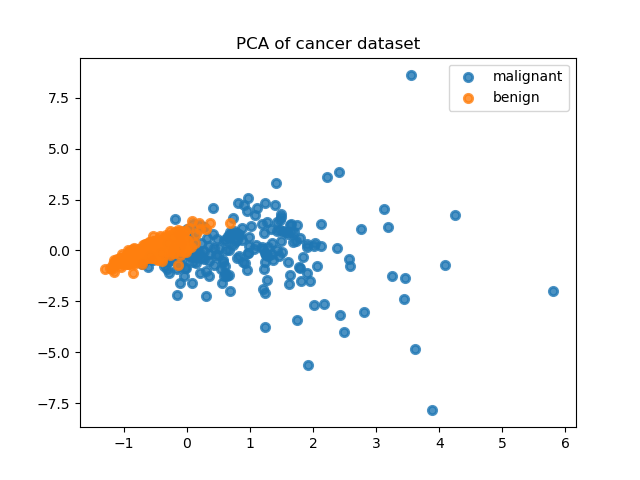
\includegraphics[scale=0.5]{images/cancer_PCA.png}
				\caption{PCA Clustering of the Breast Cancer Dataset. Visually, we can see that there is some separation, but the data lies close even after PCA.}
		\end{figure}
		
		\end{frame}
		
		\begin{frame}
			\frametitle{K Nearest Neighbors Classifier}
			
			\begin{itemize}
				\item Pre-processing:
				\begin{itemize}
					\item We split the data into a 30\% train and 70\% test sets and keep the data balanced.
					\item We also shuffle the data.
					\item We scale the data such that it is within $(0,1)$ using a min-max scaler.
				\end{itemize}
				\item The function class we consider is trivial since it is dependent only on the training data given.
				\item We can view this as a weighting function that weights the $k$-nearest points to the input with $\frac{1}{k}$ and all other points $0$.
				\item Classification Accuracy: 91 percent
				\item Training Accuracy: 94 percent
			\end{itemize}
		\end{frame}
		
		\begin{frame}
			\frametitle{Confusion Matrix for Cancer Data}
			
			\begin{figure}
				\centering
				\includegraphics[scale=0.5]{images/confusion_matrix_cancer.png}
				\caption{Confusion Matrix of Cancer Data. The data is pretty nicely classified in this binary case.}
		\end{figure}
		\end{frame}
		
		
		
		\begin{frame}
		\frametitle{Persistence Diagrams of Digits: Benign}
		
		\begin{figure}
				\centering
				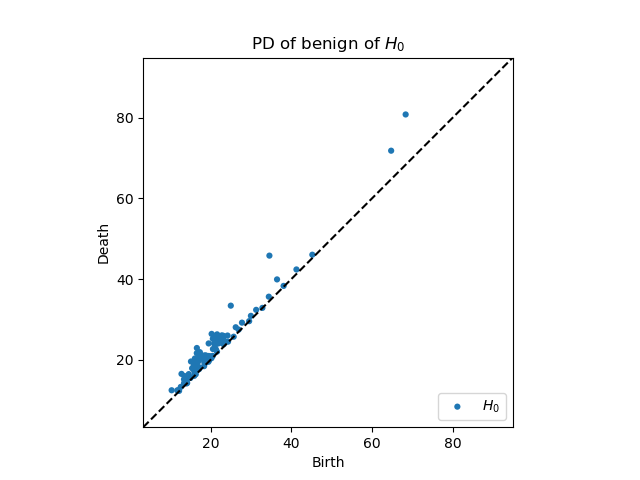
\includegraphics[scale=0.5]{images/PD_H0_benign.png}
				\caption{Persistence Diagram for Benign.}
		\end{figure}
		\end{frame}

		\begin{frame}
		\frametitle{Persistence Diagrams of Digits: Malignant}
		
		\begin{figure}
				\centering
				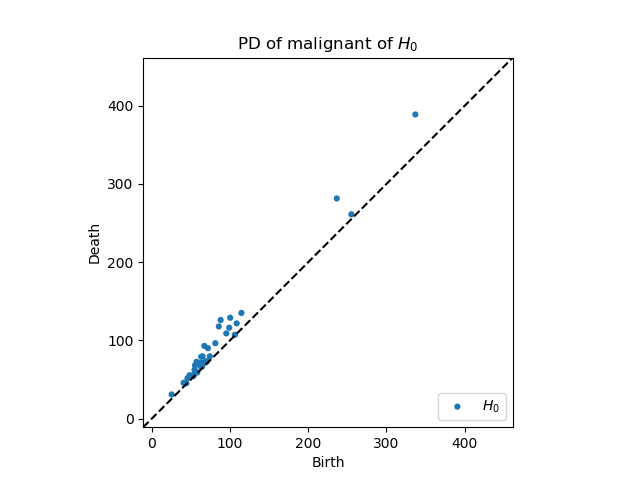
\includegraphics[scale=0.5]{images/PD_H0_malignant.png}
				\caption{Persistence Diagram for Malignant.}
		\end{figure}
		\end{frame}
		
		
		\begin{frame}
		\frametitle{Persistence Images of Digits: Benign}
		
		\begin{figure}
				\centering
				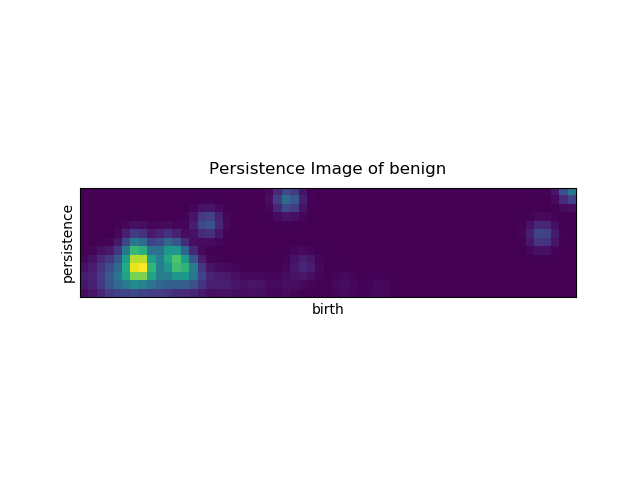
\includegraphics[scale=0.5]{images/PI_H0_benign.png}
				\caption{Persistence Image for Benign.}
		\end{figure}
		\end{frame}

		\begin{frame}
		\frametitle{Persistence Images of Digits: Malignant}
		
		\begin{figure}
				\centering
				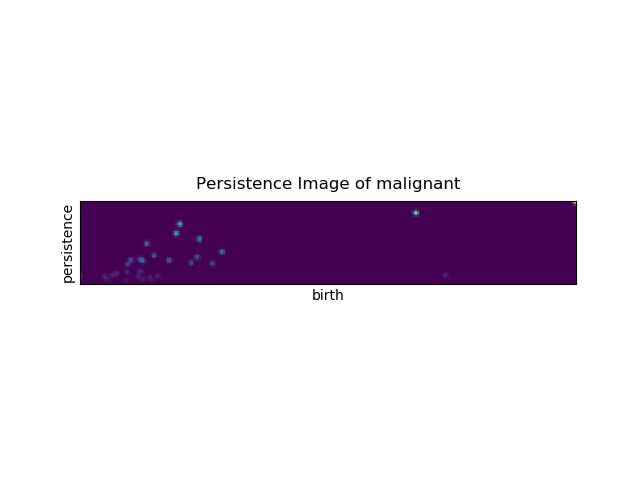
\includegraphics[scale=0.5]{images/PI_H0_malignant.png}
				\caption{Persistence Image for Malignant.}
		\end{figure}
		\end{frame}
		
		
		\begin{frame}
		\frametitle{Pairwise Bottleneck Distances}
		
		\begin{itemize}
			\item The bottleneck distances:
				\begin{itemize}
					\item With themselves: 0 (control)
					\item Benign, Malignant: 25.95355225
				\end{itemize}
		\end{itemize}
		
		A downside to the Bottleneck Distance as a measure is that quantitatively it can be hard to distinguish for simple data what a good distance is. In the binary case, unless you are comparing for hyperparameter search, this metric is close to useless.
		\end{frame}